%%%%%%%%%%%%%%%%%%%%%%%%%%%%%%%%%%%%%%%%%%%%%%%%%%%%%
\documentclass[apj]{emulateapj}
%\documentclass[preprint2]{aastex61}
%\documentclass[12pt,preprint]{aastex}
\graphicspath{{figures/}}
\DeclareGraphicsExtensions{.jpg,.pdf,.png,.eps,.ps}

\usepackage[table,usenames,dvipsnames]{xcolor}
%\usepackage{amsmath}
\usepackage{subfigure}
\usepackage[backref,breaklinks,colorlinks,citecolor=blue]{hyperref}
\usepackage{natbib}
%\usepackage{natbib}
\bibliographystyle{fapj}
\usepackage{graphicx}
\usepackage{multirow}
\usepackage{soul}

%\newcommand{\jcap}{JCAP}

\newcommand{\sqdeg}{deg$^2$ }
\newcommand{\omb}{\ensuremath{\Omega_b h^2}}
\newcommand{\omc}{\ensuremath{\Omega_c h^2}}
\newcommand{\clpp}{\ensuremath{C_{L}^{\phi\phi}}}
\newcommand{\cpmf}{\ensuremath{C_{\ell}^{\rm PMF}}}

\newcommand{\cpmftens}{\ensuremath{C_{\ell}^{\rm PMF,\,tens}}}
\newcommand{\cpmfvec}{\ensuremath{C_{\ell}^{\rm PMF,\,vec}}}
\newcommand{\apmf}{\ensuremath{A_{\rm PMF}}}
\newcommand{\bpmf}{\ensuremath{B_{\rm 1\,Mpc}}}
\newcommand{\alens}{\ensuremath{A_{\rm lens}}}
\newcommand{\lcdm}{\ensuremath{\Lambda}CDM}
\newcommand{\nrun}{\ensuremath{n_{\rm run}}}
\newcommand{\neff}{\ensuremath{N_{\rm eff}}}
\newcommand{\ho}{H\ensuremath{_0}}
\newcommand{\mnu}{\ensuremath{\sum m_\nu}}
\newcommand{\ukarcmin}{\ensuremath{\mu}{\rm K-arcmin}}
\newcommand{\lknee}{\ensuremath{\ell_{\rm knee}}}
\newcommand{\fermilat}{\textit{Fermi}-LAT}

\newcommand{\be}{\begin{equation}}
\newcommand{\ee}{\end{equation}}
\newcommand{\planck}{{\sl Planck}}
\newcommand{\wmap}{{\sl WMAP}}
\newcommand{\bicepkeck}{BICEP2/Keck Array}
\newcommand{\sptnew}{SPT-3G}
\newcommand{\pb}{\textsc{Polarbear}}
\newcommand{\simons}{Simons Array}
\newcommand{\sptpol}{SPTpol}
\newcommand{\advactpol}{Adv.~ACTpol}

\newcommand{\tbd}[1]{\textcolor{Red}{{\bf TBD}: #1}}
\newcommand{\gab}[1]{\textcolor{Orchid}{[{\bf GS}: #1]}}
\newcommand{\changed}[1]{\textcolor{Red}{#1}}
\newcommand{\removed}[1]{\textcolor{Red}{}}
\include{number_list}

%

% ref to section \S\ref{sec:label}

%\submitjournal{ApJ}
\def\Melbourne{1}
\def\uci{2}
%%%%%%%%%%%%%%%%%%%%%%%%%%%%%%%%%%%%%%%%%%%%%%%%%%%%%
\begin{document}

\title{Cosmic Microwave Background Power Spectra from Few Bit Timestreams}
\author{L.~Balkenhol\altaffilmark{\Melbourne} and C.~L.~Reichardt\altaffilmark{\Melbourne}}
\altaffiltext{\Melbourne}{School of Physics, University of Melbourne, Parkville, VIC 3010, Australia}
\email{christian.reichardt@unimelb.edu.au}

\begin{abstract}

Observations of the Cosmic Microwave Background (CMB) are of significant value to modern cosmology and particle physics. Future CMB experiments face issues in hardware design, mission planning and analysis that arise from the vast size of time-ordered-data (TOD) being recorded. These challenges are particularly significant for Antarctica- and space-based experiments which depend on satellite links to transmit their data. We explore the viability of reducing the TOD to few-bit numbers to address these issues. Unlike lossless compression, this technique introduces additional noise into the data. We present 1, 2 and 3 bit digitisation schemes and determine the degradation this compression causes in temperature and polarisation power spectra. We find that 3 bit digitisation has a percent-level contribution to the map noise level. We argue that such digitisation is a promising strategy for upcoming experiments.

\end{abstract}

%C: maybe sub techniques:misc for methods: data analysis ? unfortunately no data compression tag
\keywords{cosmic background radiation --- polarization --- techniques: miscellaneous}
\section{Introduction}
\label{sec:intro}

Observations of the Cosmic Microwave Background (CMB) have played a key role in physics since its discovery \citep{penzias1965}. Current and future CMB experiments will continue to deliver new insights by studying the temperature and polarisation information contained in the CMB. These will put tight constraints on cosmological models. Upcoming science goals include the discovery of inflationary gravitational waves, the construction of precise lensing maps and thorough studies of the Sunyaev-Zeldovich (SZ) effects. Moreover, CMB experiments will measure the relativistic number of species and the neutrino mass sum \citep{s4sciencebook}. %L: reference to science goals by satellite missions as well

High fidelity CMB science demands an excellent standard of data analysis. The CMB community has developed a variety of compression techniques and computational approaches to manage the increasing influx of data, while maximising the science output \citep{tristam2007}. These include the compression of time-ordered data (TOD) into maps \citep{tegmark1997}, bandpower estimation \citep{tegmark1998} and the pseudo $C_l$ method \citep{brown2005}.

A growing hurdle for experiments at remote locations are the transmission limitations of satellite links. Space-based experiments have employed a combination of lossless and lossy compression techniques, including reduced bits in the TOD \citep{gaztanaga1998, maris2003}. Antarctica-based experiments that transmit a portion of their data via a satellite link have downsampled their data in the past to meet their telemetry requirements. They have yet to exploit few bit digitisation of the TOD. As we approach the next generation of ground-based experiments, Stage-4, and the launch of a new generation of space-based missions (liteBIRD, PIXIE, COrE+), we must treat the transmission bottleneck carefully. Without a thorough review of compression techniques we are sure to lose information. %L:ref to non-planck satellites for reduced bit TOD? %C: Is there a reference detailing downsampling of SPT data?

In this work we present the method of extreme digitisation, which compresses a rich digital input signal into a few bits. We apply extreme digitisation to the TOD and detail its effect on temperature and polarisation power spectra. We find that an optimal 3-bit digitisation scheme adds as little as $< 2\%$ to the map noise level. The digtisation schemes described here are laid out for ground-based experiments. Space-based missions must study carefully the effect of digitisation in their specific compression algorithms.% of t the results we present here should also be considered by future space-based missions, which inevitably must incorporate lossy compression.

This work is structured as follows. In \S\ref{sec:dig} we detail the challenges originating from handling large TOD, introduce the process of extreme digitisation and lay out the framework used to test its performance. Subsequently, we describe the power spectrum estimation employed and interpret the obtained results in section \S\ref{sec:results}. We summarise our findings in \S\ref{sec:conclusions}.

%This work is structured as follows. We detail the arising challenges in handling large TOD in \S\ref{subsec:problem}. We subsequently formulate extreme digitisation in \S\ref{subsec:extremedigitisation} and lay out the framework used to test its performance in \S\ref{subsec:method}. The details of the power spectrum estimation used are laid out in \S\ref{subsec:psestimation}. We continue by presenting the noise induced through the dicitisation process in \S\ref{subsec:additionalnoise} and summarise our findings in \S\ref{sec:conclusions}. 

%CMB is great; One reason is that there is a history of compression and computational techniques that reduce the load of large datasets. ie maps; bandpowers; pseudo-cls.

%satellites have also reduced bits on TOD; ground based haven't had to yet

%however as we discuss building ever larger arrays at remote sites, we are starting to be limited: spt example.

%in this work we present digitisation for ground-based cmb polarisation measurements.
%teaser results


%The outline of this paper is as follows. 
%We present the digisation schemes in \S\ref{sec:dig}, and their performance in \S\ref{sec:results}
%We summarize our findings in \S\ref{sec:conclusions}. 

\section{Digitisation}
\label{sec:dig}

\subsection{Problem}
\label{subsec:problem}

%Data influx + Transmission

The science goals of upcoming CMB experiments naturally lead to a large influx of data To achieve the targeted sensitivity longer observations with more detectors are needed. In fact the number of detectors of ground-based experiments has been following a Moore's law like trend, doubling approximately every 2 years. This directly translates into an exponential growth in data volume \citep{s4sciencebook}. %L: check out the particle paper where the moores law figure comes from

Excellent observation conditions for CMB observations can not only be found in space, but also at various locations on earth \citep{li2017, kovac2007} among which is the South Pole. Space- and Antarctica-based experiments depend on satellite transmission. An experiment at the South Pole will be part of the next generation of ground-based instruments, which aims to collect 2 million detector years in total. Such an experiment will face a data influx of $\sim \mathrm{O}(10)\mathrm{Tb/d}$. However, the current transmission allocation for SPT3G is at $150\mathrm{Gb/d}$, which will likely only see a moderate increase in coming years. The transmission bottleneck is currently overcome by recovering the full data on hard drives with some latency and by transmitting a downsampled version of the data. The downsampling process loses high frequency information. Going into Stage-4 we anticipate that compression rates for transmission must increase by an order of magnitude. Continued use of downsampling will narrow the information window decisively - prohibiting high multipole moment science to be carried out on the transmitted data set. This also means that any potential faults or errors in the experiment that only become visible in said range will go unnoticed for longer. %L: reference for observing conditions in chile or a general review of sites %C: Is there a paper detailing trasmission limits for SPT and that the data is currently downsampled?

The Planck mission has demonstrated the merits of carrying out CMB observations from space \citep{planck2018}. Upcoming missions aim to exceed the detector count of Planck by at least an order of magnitude \citep{litebird2014, pixie2011, core2018}. However, strategies to meet the telemetry specifications of each mission appear to be in development. It is not clear whether the data compression knowledge developed during the Planck mission will guarantee optimal performance for future satellites. Most likely each mission will have to carefully construct a compression algorithm through a combination of lossless and lossy techniques, specific to their requirements.

%Planning

Beyond transmission challenges, mission planning is becoming exceedingly difficult. A full simulation of TOD over the entire parameter space of detection scenarios for numerous set-ups is the desired way to decide on Stage-4 configurations. Space-based missions must aim to carry out a similar analysis to optimise their science output. Given the shear size of TOD expected, this is not possible \citep{s4sciencebook}. We must rely on different planning strategies or aim to reduce the size of the TOD in order to maximise the productivity of planning and development stages and guarantee scientific excellence.

% Analysis

Operations on the TOD, such as noise-removal or map-making are a vital part of CMB data analysis. While we have not experienced the limitations of the accessible computational assets, the exponential growth of CMB data makes its analysis increasingly expensive. The community depends on the facilities provided by the National Energy Research Scientific Computing Center (NERSC).

%why is it worth considering

Extreme Digitisation would tackle the challenges mentioned above by reducing the size of the TOD by an order of magnitude. Together with already established lossless compression techniques (e.g. FLAC, run-length coding, Huffman coding, etc.) this will directly tackle transmission hurdles. Beyond that extreme digitisation has the potential of easing issues in planning, analysis and hardware requirements.

The Planck mission has demonstrated the advantages of using few bit compression of the TOD \citep{maris2003}. Other science areas have also shown the power of extreme digtisation. \citep{jenet1998} explored the application of such compression to radio pulsar timing measurements with success. Recently \citep{clearwater2018} have investigated the advantages of using 1 and 2 bit data when searching for continuous gravitational waves using the Laser Interferometer Gravitational-Wave Observatory (LIGO).


\subsection{Extreme Digitisation}
\label{subsec:extremedigitisation}

Digitisation is a lossy compression technique. However, the induced noise depends on the number of bits used, the digitisation thresholds, and the output levels chosen. To minimise the noise induced through this process one must know the nature of the input signal. There is usually little concern around finding an optimal set of digitisation parameters for a given input signal. It is common to have access to large numbers of bits to store information, where changes in the digitisation scheme become insignificant to the distortion induced. It is in our interest however to consider extreme, i.e. few-bit, digitisation, where a digitisation scheme must be carefully constructed. We review the key ideas regarding construction of digitisation schemes as laid out by \cite{max1960} below.

Digitisation discretises an input signal by sorting it into $N$ appropriate ranges, such that an input between $x_i$ and $x_{i+1}$ produces an output at $y_i$. The set of parameters $N, x_i, y_i$ fully specify a digitisation scheme. Conventionally one chooses $x_{1} = -\infty$ and $x_{N+1} = \infty$. In order to quantify the performance of a given digitisation scheme we define the distortion as

\begin{equation} D = \left\langle  \left( s - \hat{s} \right)^2 \right\rangle, \end{equation}

where $s$ is the input and $\hat{s}$ the output signal. For an input signal that has at least some stochastic element to it we introduce the input amplitude probability density $p(x)$. This allows us to rewrite the above as

\begin{equation} D = \sum_{i = 1}^N \int_{x_i}^{x_{i+1}} \left(x-y_i\right)^2 p(x) dx. \end{equation}

Since we wish to minimise the distortion we differentiate the above with respect to $x_i$ and $y_i$ and set the derivatives to zero. We obtain the two equations

\begin{equation} \label{eq:distderiv1}
\frac{\partial D}{\partial x_i} = \left(x_i-y_{i-1}\right)^2 p(x_i) - \left(x_i - y_i\right)^2 p(x_i) = 0,
\end{equation}

\begin{equation} \label{eq:distderiv2}
\frac{\partial D}{\partial x_j} = -2 \int_{x_i}^{x_{i+1}} \left( x-y_i \right) p(x) dx = 0.
\end{equation}

Rearranging equation \ref{eq:distderiv1} we deduce

\begin{equation} \label{eq:digitequalspacecondition}
x_i = \frac{y_i+y_{i+1}}{2},
\end{equation}

which informs us that an output level $y_i$ must lie halfway between its delimiting thresholds $x_i$ and $x_{i+1}$. From equation \ref{eq:distderiv2} we gain the additional condition

\begin{equation} \label{eq:digitareacondition}
\int_{x_i}^{x_{i+1}} \left( x-y_i \right) p(x) dx = 0.
\end{equation}

This implies that we should choose $y_i$, such that it halves the area underneath $p(x)$ in the interval from $x_i$ to $x_{i+1}$.

To progress further we have to make an assumption about the distribution of input signals, $p(x)$. For our purposes we assume that CMB observations operate at low signal to noise. Furthermore we assume that the noise profile is Gaussian white noise with standard deviation $\sigma$, i.e. $p(x) = (1/\sqrt{2\pi\sigma^2}) e^{-x^2/2\sigma^2}$. Given this assumption we can solve the problem using a numerical iterative procedure. One begins by picking $y_1$ and calculating the remaining $x_i$'s and $y_i$'s using equation \ref{eq:digitequalspacecondition}. Afterwards one checks whether this choice of values satisfy the conditions given by equation \ref{eq:digitareacondition}. If that is the case, the $x_i$'s and $y_i$'s were chosen appropriately.

We use the findings of \cite{max1960} to formulate the multi-level functions we use for our 1, 2 and 3 bit digitisation process. Given an input signal $s(t)$ a digitisation scheme using $N$ bits returns the output $\hat{s}_N(t)$. For 1 bit digitisation we apply the sign function

\begin{equation} \hat{s}_1(t) = \left\{ \begin{array}{lr}
1, & \text{for } s(t) > 0\\
-1, & \text{for } s(t) \leq 0
\end{array} \right. \end{equation}

to the TOD. For 2 bit digitisation we apply the four-level function

\begin{equation} \hat{s}_2(t) = \left\{ \begin{array}{rl}
1.51 \sigma, & \text{for } s(t) \geq 0.9816 \sigma\\
0.4528 \sigma, & \text{for } 0 \leq s(t) < 0.9816 \sigma\\
-0.4528 \sigma, & \text{for } 0.9816 \sigma \leq s(t) < 0\\
-1.51 \sigma, & \text{for } 0.9816 \sigma < s(t)\\
\end{array} \right. . \end{equation}
%C: should i round to equal significant figures here? Unfortunately these are the exact values that i used...

Finally the optimal 3 bit digitisation is described by the eight-level function

\begin{equation} \hat{s}_3(t) = \left\{ \begin{array}{rl}
2.152 \sigma, & \text{for } s(t) \geq 1.748 \sigma\\
1.344 \sigma, & \text{for } 1.05 \sigma \leq s(t) < 1.748 \sigma\\
0.756 \sigma, & \text{for } 0.501 \sigma \leq s(t) < 1.05 \sigma\\
0.245 \sigma, & \text{for } 0 \leq s(t) < 0.501 \sigma\\
-0.245 \sigma, & \text{for } 0.501 \sigma \leq s(t) < 0\\
-0.756 \sigma, & \text{for } 1.05 \sigma \leq s(t) < 0.501 \sigma\\
-1.344 \sigma, & \text{for } 1.748 \sigma \leq s(t) < 1.05 \sigma\\
-2.152 \sigma, & \text{for } 1.748 \sigma < s(t)\\
\end{array} \right. . \end{equation}

The fact that the single bit digitisation scheme makes no references to the standard deviation of the signal is irrelevant. This affects the normalisation of the signal, which we can account for later. What is important is the spacing between digitisation thresholds and relative distance between the output levels chosen.

Completely different digitisation schemes can be thought of, which would for example reference the most drastic outlier in the data set, or seek to place equal numbers of points into each digitisation level. However, given the assumptions made the schemes derived above are optimal. Additionally, they are simple enough to be easily implemented computationally.

\subsection{Methods}
\label{subsec:method}

To investigate the performance of the derived digitisation schemes we simulate many scans over CMB template maps at the timestream level. Each scan is performed by a single detector. We obtain control maps that use 64bit TOD and maps that have undergone 1, 2 and 3 bit digitisation at the timestream level. We calculate the temperature and polarisation power spectra of each map and determine the additional noise induced through the extreme digitisation process.
%C: Do I need to mention that we assume to have an infinitely fast spinning plate? %L: Check whether Python uses 32 or 64 bit under on NERSC for floats

To create the template maps we use the Hierarchical Equal Area isoLatitude Pixelization of a sphere \citep[HEALPix;][]{healpix}\footnote{Available at \url{http://healpix.sourceforge.net/}} framework. We generate a realisation of I, Q and U maps with $\mathrm{NSIDE} = 4096$ based on the results of the Planck collaboration with key cosmological parameters of $\Omega_b \approx 0.049 $, $\Omega_c \approx 0.265$, $\Omega_m \approx 0.316$ and $h \approx 0.67$ \citep{planck2016}.

%C: Do I need to comment on the fact that this reflects no particular frequency channel, but the results come from a combination of all observed channels?

We simulate observing a $\sim 600 \mathrm{deg^2}$ patch of the sky. To do so we perform a number of constant elevation scans (CES), equally spaced in declination (DEC). We repeat the observation strategy $100$ times with a slight offset in right ascension (RA) and DEC each time, such that each pixel is sampled approximately uniformly. The speed at which we sweep across the survey area is adjusted to produce a desired number of hits per pixel in the output maps.

While performing each CES the pixels being targeted are determined. The corresponding values from the template maps are then accessed and added to realisations of the detector noise of appropriate length to generate TOD streams. We assume the detector noise to be Gaussian white noise. For temperature observations we assume the detector noise level to be $500 \mathrm{\mu K \sqrt{s}}$ and for polarisation observations $\sqrt{2} \hspace{0.7ex} 500 \mathrm{\mu K \sqrt{s}}$, i.e. the corresponding photon noise limit.

At this point we apply the digitisation schemes to the TOD. We compress the timestream into maps by averaging all hits falling into the same pixel. We produce 12 CMB maps in total: three control maps (I, Q, U) and nine maps with three each obtained from each digitisation scheme.

% LINK TO GITHUB WITH CODE HERE

This process is carried out 6 times. We produce maps where pixels in the survey patch are hit approximately uniformly $800$, $8,000$, $80,000$, $1,024,000$, $10,240,000$ and $102,400,000$ times. We assume that the detector is read out $200$ times per second. %The calculation outlined above has considerable computational requirements if we want to reach up to $\sim 10^8$ hits per pixel. This calculation was made possible through use of the NERSC facilities.

%\begin{table}[tbh]
%\begin{center}
%\caption{\label{tab:inputcosparams} Input Cosmological Parameters}
%\small
%\begin{tabular}{l | c}
%Parameter & Planck 2015\\
%\hline\\begin{equation}-1.5ex]
%$100\theta_{MC}$ & $ 1.04086 \pm 0.00048$\\
%$\Omega_b h^2$ & $  0.02222 \pm 0.00023$\\
%$\Omega_c h^2$ & $ 0.1199 \pm 0.0022$\\
%$H_0$ & $67.26 \pm 0.98$\\
%$n_s$ & $0.9652 \pm 0.0062$\\
%$\Omega_m$ & $0.316 \pm 0.014$\\
%$\sigma_8$ & $0.830 \pm 0.015 $\\
%$\tau$ & $0.078 \pm 0.019$\\
%$10^9 A_s e^{-2\tau}$ & $1.881 \pm 0.014 $\\
%\end{tabular}
%\tablecomments{ 
%Cosmological parameters used to create the template maps. Taken from Planck 2015: Cosmological Parameters.
%} \normalsize
%\end{center}
%\end{table}

%\begin{table}[tbh] % transpose and include hits per pixel!
%\begin{center}
%\caption{\label{tab:modelparams} Assumed Survey Parameters}
%\small
%\begin{tabular}{l | c}
%Parameter & Value\\
%\hline \\begin{equation}-1.5ex]
%$\mathrm{NSIDE}$ &$4096$\\
%$f_{\mathrm{readout}} [\mathrm{Hz}]$ &$200$\\
%$f_{{\mathrm{sky}}}$ & $\sim 0.014$\\
%$\sigma^{\mathrm{T}}_{\mathrm{det}} [\mathrm{\mu K \sqrt{s}}]$ &$500$\\
%$\sigma^{\mathrm{Pol}}_{\mathrm{det}} [\mathrm{\mu K \sqrt{s}}]$ & $\sqrt{2}\times500$\\
%\multirow{2}{*}{$\mathrm{hits per pixel}$} & $\left(1, 10, 100 \right) \times 800,$\\
%& $\left( 1, 10, 100 \right) \times 1024000$ \\
%\end{tabular}
%\tablecomments{ 
%Parameters used in the simulated observation. The RA speed is adjusted to match the desired hits per pixel.
%} \normalsize
%\end{center}
%\end{table}



\section{Results}
\label{sec:results}

\subsection{Power Spectrum Estimation}
\label{subsec:psestimation}

We use the Spatially Inhomogeneous Correlation Estimator for Temperature and Polarisation \citep[PolSpice;][]{polspice} to compute the $\mathrm{TT}, \mathrm{EE}$ and $\mathrm{BB}$ power spectra of the reconstructed maps I, Q, U maps. To minimise cut sky effects we apodise the observed path using a cosine mask with $\sigma_{\mathrm{APOD}} = \sqrt{600}/2 \hspace{0.7ex} \mathrm{deg}$. %C: Should I also mention the multiplication with a cosine mask that I supply in addition to setting this option on polspice? This will likely be reworked when using Healpix to get the power spectra though.

%%%%%%%%%%%
% INCLUDE SECTION OF ALM CUTS (maybe a plot of the cuts too)
%%%%%%%%%%%


%\begin{table}[tbh]
%\begin{center}
%\caption{\label{tab:polspiceparams} PolSpice Parameters}
%\small
%\begin{tabular}{c c c c}
%weights & $\sigma_{\mathrm{APOD}} [\mathrm{deg}]$ & apodistation type & polarisation \\
%\hline
%cosine mask & $\sqrt{600}/2$ & cosine & Yes \\
%
%\end{tabular}
%\tablecomments{ 
%Parameters used when calling PolSpice to calculate the power spectra. Remaining parameters have been left at their default value.
%} \normalsize
%\end{center}
%\end{table}


%%%%%%%%%%%
% THIS MIGHT CHANGE WHEN WORKING OUT THEORETICAL NORMALISATION
%%%%%%%%%%%

Normalisation of the obtained power spectra is necessary. The digitisation schemes introduced in section \S\ref{sec:dig} are designed to minimise the distortion of the TOD, not to preserve power at the map level. Normalising obtained spectra against previous experiments is a common calibration technique in many CMB experiments (e.g. SPT). %C: Do you know a good reference for this?

For the normalisation procedure we focus on the $\sim 10^8$ hits per pixel maps. We normalise the $\mathrm{TT}$, $\mathrm{EE}$, and $\mathrm{BB}$ power spectra from few bit TOD against their control counterparts. We consider the normalisation window cut out by the conditions

\begin{equation} l > 35 \> , \> \frac{C_l^{\mathrm{S}}}{C_l^{\mathrm{N}}} \geq 10. \end{equation}

where $C_l^{\mathrm{S}}$ is the power spectrum of the input template maps and $C_l^{\mathrm{N}}$ the detector noise level. The lower limit is placed in accordance to the patch-size surveyed while the upper limit ensures appropriate signal to noise in the normalisation window.

The normalisation constants for each digitisation scheme and channel obtained through this way are then applied to all lower hits per pixel simulations. A sample of the obtained power spectra is shown in figure X.

%%%%%%%%%%%
%SAMPLE POWER SPECTRA WITH THEORY SPECTRA
% want to show that we recover the PS, including theory PS in background
%%%%%%%%%%%

%\begin{figure}[htb]\centering
%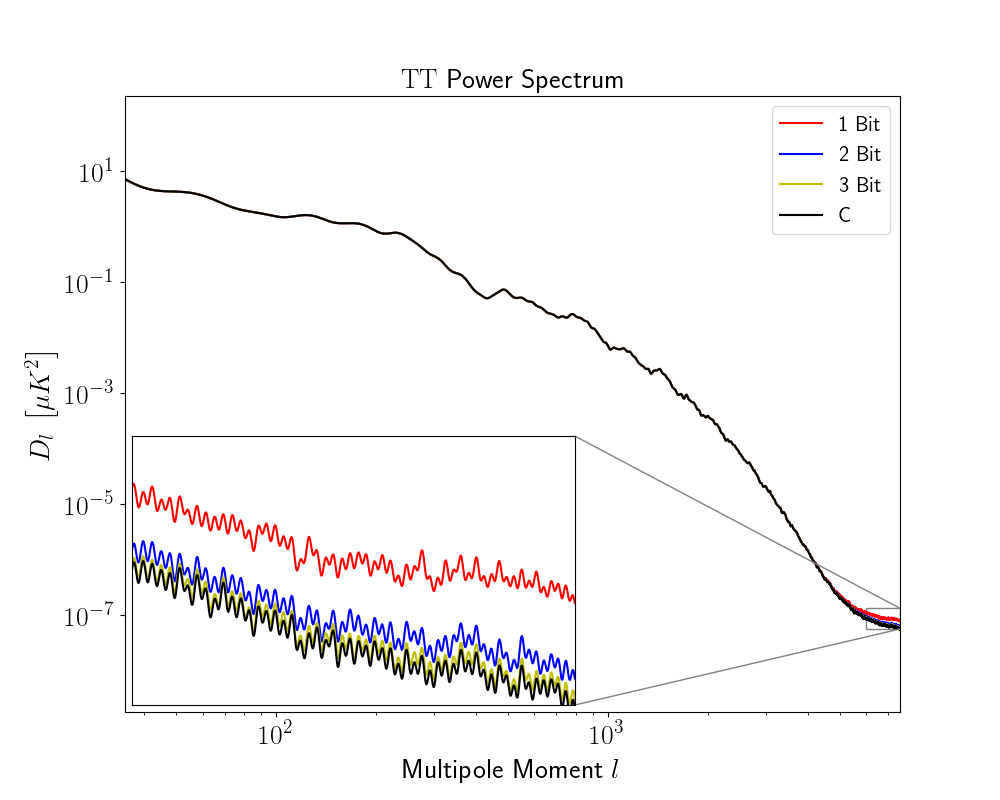
\includegraphics[width=0.5\textwidth,clip]{Plots/ttzoom.png}
%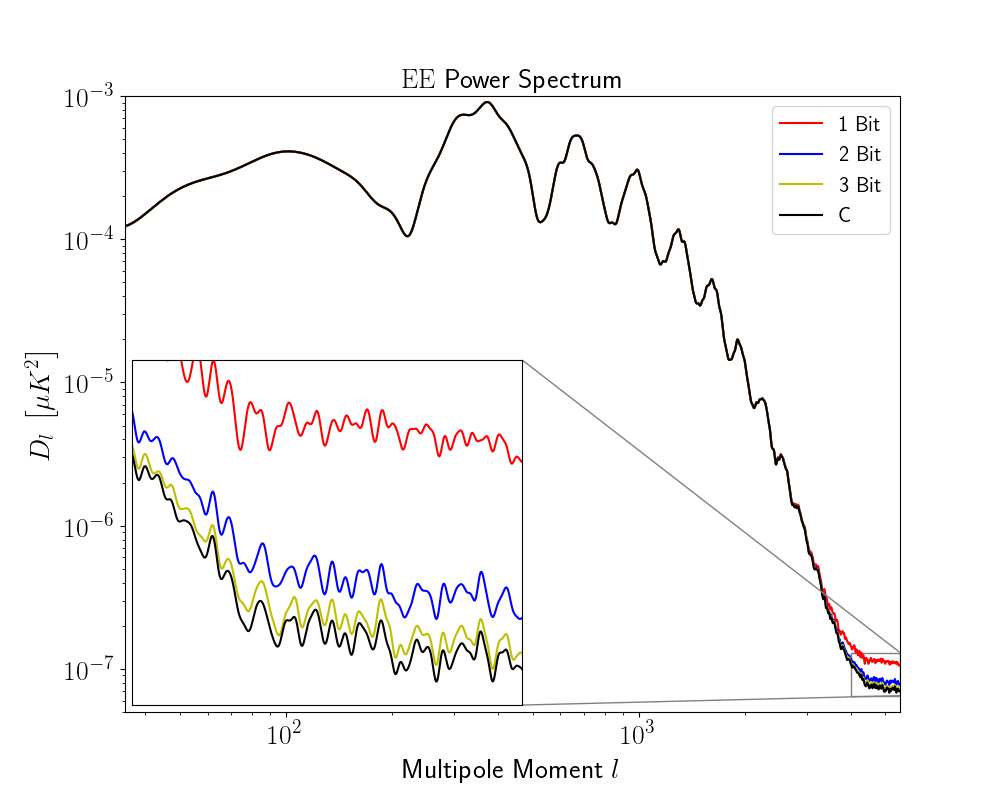
\includegraphics[width=0.5\textwidth,clip]{Plots/eezoom.png}
%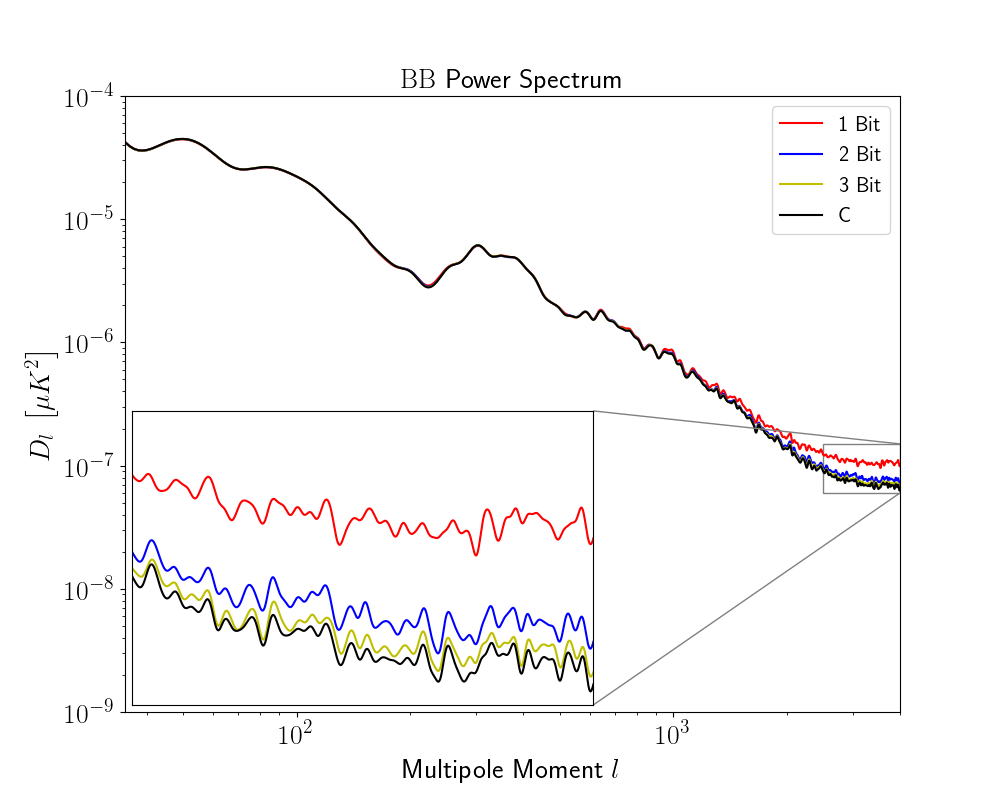
\includegraphics[width=0.5\textwidth,clip]{Plots/bbzoom.png}
%  \caption[Current ]{
%   Reconstructed $\mathrm{TT}$, $\mathrm{EE}$, and $\mathrm{BB}$ power spectra. These originate from an observation with $102400000 \mathrm{hits per pixel}$. We observe that digitisation appears to add some constant to the noise level. As one would expect $3 \mathrm{Bit}$ digitisation performs the best, followed by $2 \mathrm{Bit}$- and finally $1 \mathrm{Bit}$ digitisation.
%\label{fig:powspeczoom}
%}
%\end{figure}


\subsection{Additional Noise}
\label{subsec:additionalnoise}

%C: This is where I'm planning on
%%%%%%%%%%%
% INSERT A COUPLE PARAGRAPHS ABOUT THE PS OF DIFFERENCE MAPS
% INCLUDE PLOTS OF PS OF DIFFERENCE MAPS
% want to show that beyond some calibration error, we do not observe any l dependence in the added noise
%%%%%%%%%%%

To quantify the distortion caused by extreme digitisation we infer the map noise level from the relevant power spectra. These are put into the context of the map noise level deduced from the control power spectra. We formulate

\begin{equation} \label{eq:extramapnoise}
\frac{\Delta \sigma}{\sigma} = \frac{\sigma_{\mathrm{map}}^{\mathrm{D}}-\sigma_{\mathrm{map}}^{\mathrm{C}}}{\sigma_{\mathrm{map}}^{\mathrm{C}}},
\end{equation}

where $\sigma_{\mathrm{map}}^{\mathrm{C}}$ is the map noise level of the control power spectra and $\sigma_{\mathrm{map}}^{\mathrm{D}}$ is the map noise level obtained from the power spectra originating from extremely digitised TOD. We assume that the digitisation process results in adding a constant noise term to each power spectrum. If we are dominated by noise we can write

\begin{equation} C_l^\mathrm{D} \approx C_l^\mathrm{N} + C_l^\mathrm{X}. \end{equation}

Here $C_l^\mathrm{D}$ is the total power spectrum originating from a digitised timestream and $C_l^\mathrm{X}$ the additional noise induced through digitisation. We now progress equation \ref{eq:extramapnoise} to

\begin{equation}\frac{\Delta \sigma}{\sigma} = \sqrt{\frac{C_l^\mathrm{D}}{C_l^{\mathrm{N}}}} - 1 = \sqrt{1 + \frac{C_l^\mathrm{X}}{C_l^{\mathrm{N}}}} - 1 . \end{equation}

% = \sqrt{\frac{C_l^N + C_l^X}{C_l^{N}}} - 1 

The value of $l$ at which we can safely assume to be noise dominated and apply the above framework varies between simulated observations of different hits per pixel and temperature and polarisation power spectra. To define the range of noise domination we choose the condition

\begin{equation} \frac{C_l^{\mathrm{N}}}{C_l^{\mathrm{S}}} \geq 10. \end{equation}

Before analysing $C_l^\mathrm{X}/C_l^\mathrm{N}$ we rebin the power spectra to $\Delta l \approx 100$. This guarantees that the points in the noise tail are independent of one another, allowing us to extract an uncertainty for the above quantity.% Plots for $C_l^\mathrm{X}/C_l^\mathrm{N}$ are shown in figure X.% l = 123 at the moment

%\begin{figure}[htb]\centering
%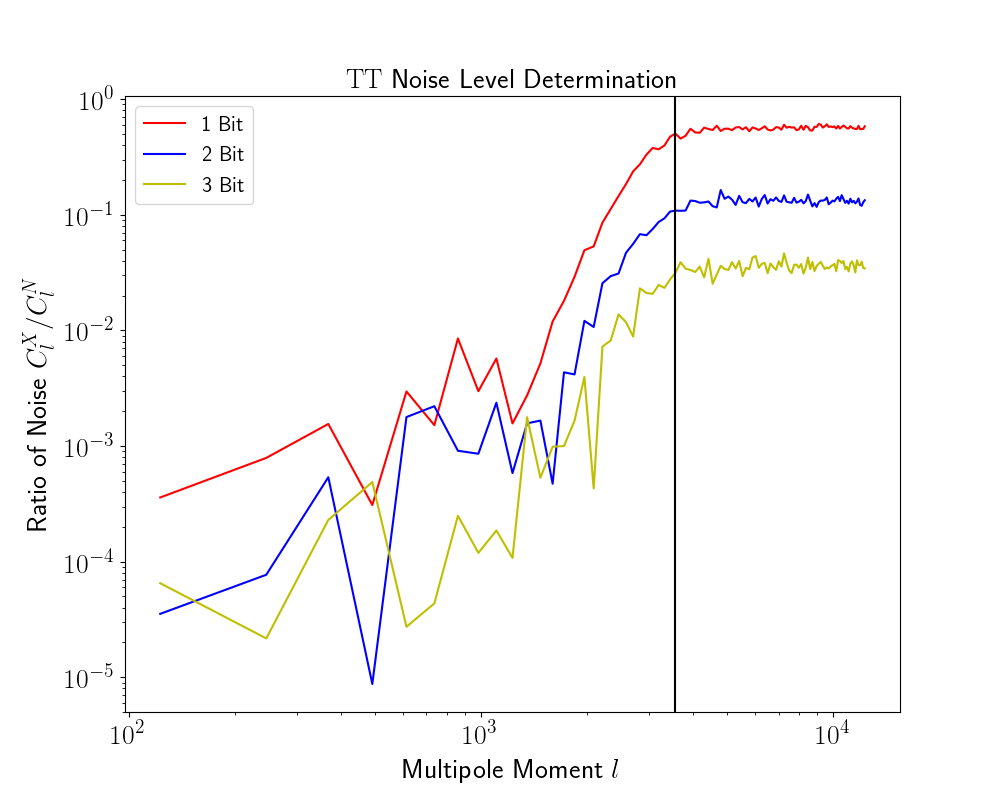
\includegraphics[width=0.5\textwidth,clip]{Plots/ttratio.png}
%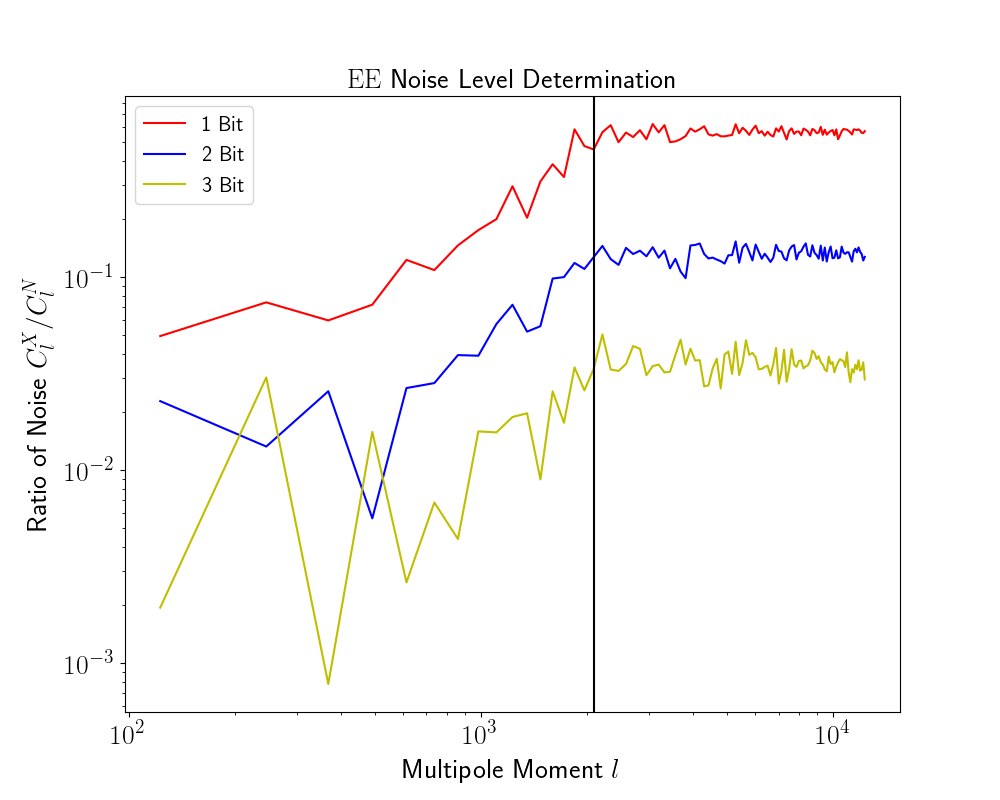
\includegraphics[width=0.5\textwidth,clip]{Plots/eeratio.png}
%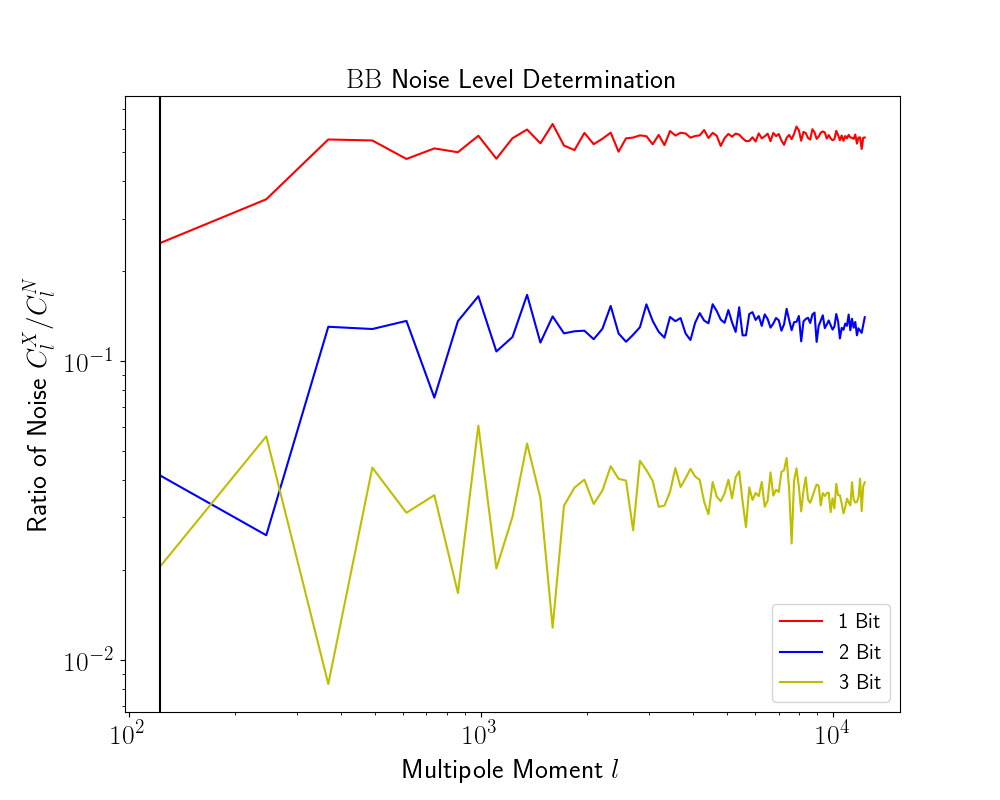
\includegraphics[width=0.5\textwidth,clip]{Plots/bbratio.png}
%  \caption[Current ]{
%  Calculated ratio of $C_l^\mathrm{X}/C_l^\mathrm{N}$ of the rebinned $\mathrm{TT}$, $\mathrm{EE}$, and $\mathrm{BB}$ power spectra. The vertical black line indicates from which point onwards data is used to calculate the equivalent noise level. The above power spectra originate from a $80000\mathrm{hits per pixel}$ map. Increasing the hits per pixel in the map shifts the plateau to the right.
%\label{fig:clxcln}
%}
%\end{figure}

The deduced additional noise for 1, 2 and 3 bit digitisation schemes are shown with respect to the hits per pixel in the maps in table \ref{tab:extranoise}. We would like to point out the following key results. Firstly, 3 Bit digitisation performs the best, followed by 2 Bit and finally 1 Bit digitisation. This is what we expect, given that with each additional bit we retain more information. For a fixed detector noise level the deterioration of the map quality scales in the same fashion as the number of hits per pixel. We see that $\Delta \sigma / \sigma$ is independent of the hits per pixel in the maps. Furthermore, the compression works equally well for temperature as it does for polarisation observations. Lastly, the added noise levels are astonishingly low. The optimal 3 Bit digitisaiton scheme devised adds as little as $<2\%$ to the map noise level. Keeping in mind that CMB detector sensitivity improves in steps of order of magnitude every few years, adding an extra percent-level noise term does not deteriorate the results appreciably. This is impressive, given that the use of an optimal 3 bit digitisation scheme will save approximately an order of magnitude in TOD volume.

\def\arraystretch{1.2}
\begin{table*}[tbh]
\begin{center}
\caption{\label{tab:extranoise} Additional Noise}
\small
\begin{tabular}{c c c c c}
Hits Per Pixel & Channel & 1 Bit & 2 Bit & 3 Bit \\
\hline
\hline
\multirow{3}{*}{800}  & TT  & $ 0.252 \pm 0.009 $  & $ 0.064 \pm 0.003 $  & $ 0.017 \pm 0.002 $ \\
& EE  & $ 0.252 \pm 0.012 $  & $ 0.064 \pm 0.005 $  & $ 0.017 \pm 0.004 $ \\
& BB  & $ 0.252 \pm 0.011 $  & $ 0.066 \pm 0.005 $  & $ 0.018 \pm 0.004 $ \\
\hline
\multirow{3}{*}{8000}  & TT  & $ 0.252 \pm 0.007 $  & $ 0.064 \pm 0.003 $  & $ 0.017 \pm 0.002 $ \\
& EE  & $ 0.252 \pm 0.007 $  & $ 0.064 \pm 0.004 $  & $ 0.017 \pm 0.002 $ \\
& BB  & $ 0.25 \pm 0.018 $  & $ 0.064 \pm 0.009 $  & $ 0.018 \pm 0.004 $ \\
\hline
\multirow{3}{*}{80000}  & TT  & $ 0.249 \pm 0.011 $  & $ 0.064 \pm 0.005 $  & $ 0.018 \pm 0.002 $ \\
& EE  & $ 0.25 \pm 0.011 $  & $ 0.064 \pm 0.005 $  & $ 0.018 \pm 0.002 $ \\
& BB  & $ 0.247 \pm 0.018 $  & $ 0.064 \pm 0.009 $  & $ 0.018 \pm 0.004 $ \\
\hline
\multirow{3}{*}{1024000}  & TT  & $ 0.25 \pm 0.009 $  & $ 0.063 \pm 0.003 $  & $ 0.017 \pm 0.002 $ \\
& EE  & $ 0.252 \pm 0.008 $  & $ 0.065 \pm 0.003 $  & $ 0.018 \pm 0.002 $ \\
& BB  & $ 0.251 \pm 0.008 $  & $ 0.064 \pm 0.004 $  & $ 0.018 \pm 0.002 $ \\
\hline
\multirow{3}{*}{10240000}  & TT  & $ 0.186 \pm 0.025 $  & $ 0.047 \pm 0.007 $  & $ 0.013 \pm 0.002 $ \\
& EE  & $ 0.252 \pm 0.009 $  & $ 0.064 \pm 0.004 $  & $ 0.018 \pm 0.002 $ \\
& BB  & $ 0.25 \pm 0.012 $  & $ 0.065 \pm 0.005 $  & $ 0.018 \pm 0.002 $ \\
\hline
\multirow{3}{*}{102400000}  & TT  & $ 0.246 \pm 0.004 $  & $ 0.063 \pm 0.002 $  & $ 0.017 \pm 0.001 $ \\
& EE  & $ 0.251 \pm 0.008 $  & $ 0.064 \pm 0.004 $  & $ 0.017 \pm 0.002 $ \\
& BB  & $ 0.251 \pm 0.009 $  & $ 0.065 \pm 0.003 $  & $ 0.018 \pm 0.002 $ \\
\end{tabular}
\tablecomments{ 
Percent addition to the map noise level $\Delta \sigma / \sigma$ by digitisation. Notice the invariance for each digitisation scheme with the number of hits per pixel and channel.
} \normalsize
\end{center}
\end{table*}

Extreme digitisation is a viable lossy compression technique when dealing with low signal to noise, large data sets with a signal that is slowly varying with respect to the sampling rate. Under these conditions we have a locally flat, small signal, on top of which we add many large noise realisations. These conditions allow us to reconstruct the underlying signal well. Furthermore a small signal will prevent saturation of the output, i.e. the inability of the digitised output to represent numbers larger than $y_N N_{\mathrm{hit}}$ or smaller than $y_1 N_{\mathrm{hit}}$, where $N_{\mathrm{hit}}$ is the number of data points in a given interval.

%communicate any information where in the first and last digitisation range ( $\left(x_N, \infty \right)$ and $\left( -\infty, x_1 \right)$ )the input signal lies.

%Extreme digitisation is a viable lossy compression technique when dealing with large volume, low signal to noise, slowly varying datasets. Making these assumptions the signal is small and constant for a considerable number of datapoints. For such an interval many samplings of the signal plus noise result in producing appropriate numbers in each output bin. The addition of more bits helps by classifying the size of the noise more accurately and hence approaching an improved estimate for the value of the signal faster. It is necessary to remain in the low signal to noise regime, as otherwise a dominant signal would saturate the digitisation scheme and for a given scheme only values in the range $\pm |N_{\mathrm{hits}}y_N|$ can be represented, given that we have $N_{\mathrm{hits}}$ datapoints. We must demand the data to be slowly varying such that many datapoints can be used to reconstruct a single significant step of the input signal. Finally a large data volume is clearly favourable for the reasons illustrated above: it allows for repeated sampling and therefore more accurate reconstruction of the weak signal.

%\begin{table*}[tbh]
%\begin{center}
%\caption{\label{tab:experiments} Assumed survey parameters}
%\small
%\begin{tabular}{l || c c c c c }
%Experiment & Sky coverage & Polarized Noise level  & 1/$f$ knee & Beam FWHM \\
%& &($\mu$K-arcmin)&&(arcmin.)\\
%\hline
%\tiny \\ \small
%CMB Stage III & & & & \\
%~~~~~SPT-3G & 6\% & 3.0 & 200 & 1.2 \\
%~~~~~Simons Array & 36\% & 9.5 & 200 & 3.5 \\ 
%\tiny \\ \small
%\hline
%CMB Stage IV & 55\% & 1.3 & 100 & 4.0 \\
%\end{tabular}
%\tablecomments{ 
%Key numbers about the planned stage III and IV experiments. 
%The sky coverage percentages are after galactic cuts. 
%Unless otherwise noted,  the Fisher matrix forecasts in this work use these numbers. 
%All forecasts also allow for beam and calibration uncertainties as noted in the text. 
%} \normalsize
%\end{center}
%\end{table*}

\section{Conclusion}
\label{sec:conclusions}

In this work we have motivated the investigation of extreme digitisation as a technique in combating arising challenges in CMB data analysis. The reduction of TOD by an order of magnitude directly addresses issues in transmission faced by remote location observations. Benefits in mission planning, data analysis and hardware requirements are possible.

We derived a set of optimal 1, 2 and 3 bit digitisation schemes assuming white detector noise. Through simulated observation we determined the distortion this compression technique causes in temperate and polarisation power spectra. We find that an optimal 3 bit digitisation adds as little as $<2\%$ to the map noise level for temperature and polarisation observations alike. No change in the results is observed for maps of different hits per pixel. The additional noise is insignificant given that the sensitivity of CMB experiments follows a Moore's law like trend, improving by orders of magnitude between generations. %L: Comment about invariance with multipole moment

Future work investigating this compression technique must aim to understand the nature of the induced noise better. It is of great value to find the higher statistical moments, i.e. skewness and kurtosis, of the added noise term. For this an analysis of the performance of cluster-finding algorithms on the digitised TOD is considered useful.

%It should be laid out how the results changes when moving to a more realistic noise profile. We do not expect this to alter the practicality of our results - even if a different noise profile doubles the additional percentage to the map noise level extreme digitisation is still practical. Ideas on how to deal with 1/f noise, e.g. chunking of the data before applying extreme digitisation have already been investigated by Planck. These thoughts should be considered when designing the compression schemes of future space-based CMB missions, which will be unable to recover their full data with latency, but rely entirely on the transmitted information.

\acknowledgments % thank patrick for discussion/starting point? Andrew?

% Melbourne CMB group, funding, NERSC.

We thank the \changed{referee as well as} Srinivasan Raghunathan and Federico Bianchini for valuable feedback on the manuscript. 
We acknowledge support from an Australian Research Council Future Fellowship (FT150100074), and also from the University of Melbourne. 
This research used resources of the National Energy Research Scientific Computing Center, which is supported by the Office of Science of the U.S. Department of Energy under Contract No. DE-AC02-05CH11231. 
We acknowledge the use of the Legacy Archive for Microwave Background Data Analysis (LAMBDA). Support for LAMBDA is provided by the NASA Office of Space Science.

% all code stuff

This research made use of the NumPy \citep{numpy}, SciPy \citep{scipy}, Matplotlib \citep{matplotlib}, and Astropy \citep{astropy} packages available for Python.


\bibliography{digitisation}


\end{document}
